\documentclass{article}
\usepackage[utf8]{inputenc}
\usepackage{graphicx}

\title{Learning Journal}
\author{Sophie Wallace }
\date{August 2019}

\begin{document}

\maketitle
\tableofcontents


\section{10/08/2019}
\subsection{Thoughts/Intentions}

\textbf{11:04am}: I’m currently downloading LaTeX and beginning the Data Carpentry exercise for this week. Finding the various different applications very overwhelming and hoping that after the exercises I will have a clearer idea of it all. 


\textbf{11:30am}: Found out from a friend that I don’t have to download MacTeX/LaTeX onto my computer for four hours and now going to go to overleaf instead. 


\textbf{11:57am}: Decided before completing Data Carpentry exercise, I want to familiarise myself with Overleaf and Github. Currently learning how to use GitHub and create a repository 


\textbf{12:30pm}: After having complications with Overleaf, now returning to Data Carpentry exercise and writing notes in cloudstor weekly journal. 

\subsection{Action}

\begin{itemize}
\item Clicked the link to download MacTeX 2019 on the LaTeX website, downloading time is estimated at 2-3hours. 
\item Entered into Introduction for Data Organization in Spreadsheets for Social Scientists
\item Cancelled LaTeX download and opening Overleaf. 
\end{itemize}



Creating a repository on Github:

\begin{itemize}
\item Click on profile icon in top right corner and click ‘your repositories’
\item Click ‘new’ and entering details - named repository ‘learning-journal’
\item Selected initialize this repository with a README and created repository
\item Uploading overleaf weekly template sample
\item Commited file with description
\end{itemize}
 
Overleaf:
\begin{itemize}
\item Used sample template in Overleaf and edited title/abstract - recompiled and downloaded pdf for Github.
\item Copy and pasted text from cloudstor document to new file in overleaf
\item Attempt to recompile presents \textbf{ERROR} - still recompiles to the weekly journal template. 
\item Deleted template and recompile section dissapeared with \textbf{ERROR} - “Unknown main document. Please choose the main file for this project in the project menu”
\end{itemize}

Data Carpentry Exercises:

\textit{Messy Spreadsheet}

\begin{itemize}
\item Opened data sets from previously downloaded excel spreadsheets
\item Found ‘tabs’ in excel in bottom left corner
\item Discussing messy data
\item Color used for indication
\item Multiple variables in column and row
\item Multiple values in single cells
\item Inconsistencies in null, 0 and false in each tab
\item Inconsistencies and use of asterisk
\item Blank cells are not adequate indicators
\item Multiple tabs in one spreadsheet
\end{itemize}

\textit{Metadata }


\begin{itemize}
\item Unclear data
\item There seems to be a reoccurring and limited representation of items owned. Is there a specific criteria for items to be recorded?
\item What does no to member associations exactly mean? That the members in the household are recluse or separate from the society they are living in?
\item What is the question and context for ‘affect-conflict’ - what affects the conflict?
\item Does years-liv refer to years lived in the house or community?
\end{itemize}


\textit{Formatting Problems}

\begin{itemize}
\item Use ‘blank’ for a null value - best option
\item Use (underscores) for spaces in between words i.e. formatting(underscore)problems
\end{itemize}\subsection{Results}

\begin{itemize}
\item Github - new repository named learning-journal with practice upload committed. 
\item Overleaf - very confused, do not have a document to work with that is in pdf format. Leaving for now, will continue journal in cloudstor and will ask for assistance in class. 
\item Data Carpentry - straight forward and informative exercises. Completed up until Formatting problems.
\end{itemize}

\subsection{Final Thoughts}

\textbf{2:03pm}: I feel a lot more confident with cloudstor and data carpentry however using github and overleaf will take a lot more practice and hopefully some assistance. Satisfied with the progress today and I will complete the scoping exercise tomorrow morning.


\section{11/08/2019}

\subsection{9am Problematic Data in Anthropology}

Problematic data surrounding the discipline of anthropology include the often tumultuous and unexpected occurrences that happen during fieldwork, as well as the collection of accurate data and removing all bias from cultural interpretations. University employers and funding agencies have recently been demanding for accountability in data management from anthropologists, which creates a concern for the ethical governance of social relationships and participants in the field (Pels et al, 2018).



Examples of problematic data in an anthropological context would be the highly inter subjective and iterative process that fieldwork and ethnography encapsulate. Therefore, anthropologists should make an epistemological distinction between ‘raw’ data and ‘processed’ data to encourage transparency and limit bias. Another instance of problematic data would be the heightened ethical concerns that anthropologists must be aware of and counter when processing or presenting data for transparency. Therefore anonymity can be an integral part when writing data. This can create messy or problematic data due to the lack of accuracy, detail and accountability being removed from materials to ensure ethical consideration. 



Pels, P., Boog, I., Henrike Florusbosch, J., Kripe, Z., Minter, T., Postma, M., Sleeboom-Faulkner, M., Simpson, B., Dilger, H., Schönhuth, M., von Poser, A., Castillo, R., Lederman, R. and Richards-Rissetto, H. (2018). Data management in anthropology: the next phase in ethics governance?. Social Anthropology, 26(3), pp.391-413.

\section{11/08/2019}

\subsection{Thoughts/Intentions}

\begin{itemize}
\item \textbf{10:02am}: Beginning scoping exercise and hoping to complete in Overleaf
\item \textbf{11:30am}: Just confirmed my email with overleaf and added MQ affiliation. Now attempting to link overleaf with my github account
\end{itemize}

\subsection{Action}

Scoping Exercise

\begin{itemize}
\item Open scoping exercise in cloudstor
\item Open blank document in overleaf
\item Written introduction under intro section then created a new section
\item Recompiled document 
\item Opened “A day in the life worksheet”
\item Finished jobs section and created new section using pains
\item Repeated section command for pain relievers
\item ERROR in Overleaf - unable to make the first point under the section in line with the reset of the points.
% BBS: \ means something special. To have it output \ you need to "escape" it as per https://en.wikibooks.org/wiki/LaTeX/Special_Characters 
% BBS: Also, for quotes, if you want them to be "fancy" (in terms of appearing to curve up at the start and down at the end, LaTeX wants you to use `` and '' (or ` and ' for single quotes)
\item Attempted more line spaces and finding a command in ``\\'' to correct however unsuccessful - will ask in class
\item Completed document and saved as PDF
\item Uploading to cloudstor Sophie Wallace Scoping Exercise folder.
\item Made new repository in github under scoping-exercise 
\item Added description and committed with a README
\end{itemize}


Overleaf —> Github

\begin{itemize}
\item Found github sync command in left Menu tab on overleaf
\item Clicked authorise and was met with “This project is not linked to a GitHub repository. You can create a repository for it in GitHub”
\item Now following button to ‘create github repository’
\item Opens export project to github and asks to create new repository with description
\item Created and clicked ‘public’ option
\item \textbf{ERROR}: repository creation failed “please check that the repository name is valid,  and that you have permission to create the repository.
\item \textbf{FIXED}: Changed the name scopingexercise and worked - error may have been in creating a repository with the exact same name as a previous one.
\item I now have two repositories with scoping exercises
\end{itemize}

\subsection{Final Thoughts}

\textbf{11:49am}

\begin{itemize}
\item Scoping exercise: I found this exercise to be relevant and thought-provoking in how I can utilize this unit in making my thesis easier to manage and organize. It was straight forward and interesting. 
\item Overleaf: I’m glad Overleaf worked for me this time and I was able to successfully create a document. I would still love to learn how to properly format and become comfortable with utilizing its features. 
\item Github: Although I am able to upload and create repositories, I don’t think I have a full grasp of its features or process. I also do not think that I am connected to a shared FOAR705 github so I will need to figure that out in class.
\item Cloudstor: very straightforward and easy to use.
\end{itemize}

\section{18/06/2019}
\subsection{Thoughts/Intentions}
\textbf{7:40pm}:  I've set up another monitor on my desk to help with the multiple tabs that need to opened at once and feeling more organized. Planning to work through data carpentry.

\textbf{9:05pm}: I want to quickly try again at the data sheet after reading other students processes for this task in their learning journals. 

\subsection{Action}

Dates as Data 
\begin{itemize}
\item Open 'Dates as Data' section in 'Data Organization in Spreadsheets for Social Sciences'
\item Downloaded SAFI dated spreadsheet
\item Had to google "how to extract components of date into new columns" because I was unsure what this meant (novice excel user here)
\item Created new columns adjacent to interview dates and named each column "day" , "month", "year" 
\item Wrote in Day column next to interview date 17/11/2016 =DAY(17) 
\item \textbf{ERROR}: the cell automated to 17/01/1900
\item Wrote in the month column =MONTH(11) - \textbf{ERROR}: automated to 01/01/1900
\item Retyped under Day column =Day(B2) to refer to the date - \textbf{ERROR}: There are one or more circular references where a formula refers to its own cell either directly or indirectly. This might cause them to calculate incorrectly.
\item Re-downloading spreadsheet and starting fresh.
\item \textbf{ERROR} - same issue where =day(17) automates to 17/01/1900
\item Filling it all out with the automated system, I see that the excels date systems (1990) is meant to be relevant, I'm confused to how it applies but will ask.
\item Just noticed the solution tab on Data Carpentry and going to enter dates manually without an automated function and ask question in class.
\item Added formula to each column underneath i.e. day column has =day(b1:b15)
\item \#VALUE! appears in the formula cell. 
\item Leaving for now.
\end{itemize}

Dates as Data (Attempt 2)

\begin{itemize}
\item Opened new spreadsheet 
\item Remembered to create a new tab rather than to manipulate the raw data
\item Copied interview dates into column A in new tab
\item Named column B - Day, column C - month and column D - year
\item Entered the formula =day(A2) into B2 -\textbf{ SUCCESS}
\item Clicked and dragged the bottom right corner of cell B2 down entire column
\item Day column has now extracted the dates correctly.
\item Copying process with month and year column -\textbf{SUCCESS}
\item Adding 17/11 in cell A16, automates to 17-Nov in interview date section and includes the year 2019 in the column
\item If no year is specified the current year must be inserted.
\item End of dates as data exercise.

\end{itemize}

\subsection{Final Thoughts}
\textbf{8:30pm} Very frustrating that what was assumed as a simple task has taken a lot of back and forth and time but hoping once I'm able to reiterate these errors with someone it will be clear and straight forward. 


\textbf{9:22pm} After reading through other learning journals it became a lot clearer the mistakes I was making. I wish there were clearer instructions in these sites to assist with novice users such as myself. I am glad that I was able to successfully complete the exercise after seeing similar steps. This task reminded me that I must use a new tab when adding and working with data in excel. 

\section{22/08/2019}
\subsection{Thoughts/Intentions}
\begin{itemize}
\item \textbf{10:02am}: Creating a readme for the learning journal on github
\item \textbf{10:06am:} Track action of committing overleaf version to github
\item \textbf{12:09pm} Finishing data carpentry
\item \textbf{12:21pm} Complete quality assurance exercise to apply new validation rule
\item \textbf{1pm} Complete excel data export exercise
\end{itemize}


\subsection{Actions}
ReadMe Github
\begin{itemize}
\item Entered into learning journal repository on github
\item Clicked pencil edit icon 
\item Entered description in file section 
\item Entered readme name and description in commit changes section
\item Committed changed \textbf{SUCCESS}
\end{itemize}

Version Control
\begin{itemize}
\item After recompiling overleaf document, enter menu section in top left corner
\item Click "github" in sync section
\item Click "push overleaf changes to github"
\item Commited \textbf{SUCCESS}

\end{itemize}
Data Carpentry 
\begin{itemize}
\item Created a copy of raw data in new tab under DC Exercises
\end{itemize}

\textit{Quality Assurance Exercise}
\begin{itemize}
\item Selected rooms column
\item Clicked data tab
\item Selected data validation
\item Selected whole number
\item Entered minimum of 1 and maximum of 25
\item Clicked on input message 
\item Named title - invalid number
\item Input message - number of rooms must be a whole number between 1 and 15
\item Tested violation of the data and \textbf{SUCCESS} it incurred an error.
\end{itemize}

\textit{Restricting Data Exercise}
\begin{itemize}
\item Selected village column
\item Clicked data tab
\item Selected data validation
\item Selected list in allow drop-down menu
\item Listed values separated by commas including: God, Chirodzo, Ruaca
\item Selected input message
\item Titled 'Valid Data'
\item Input message as 'Values accepted in village column are God, Chirodzo, Ruaca
\item Clicked ok
\item Tested violation of the data and \textbf{SUCCESS} it incurred an error
\end{itemize}

\textit{Exporting Data}
\begin{itemize}
\item Selecting file and save as
\item Selected comma separated values in the format field
\item Checked name and location, clicked saves
\item \textbf{ERROR}: This workbook cannot be saved in the selected file format because it contains multiple sheets. To save the entire workbook, click Cancel, then save the workbook in another format. To keep the selected format and save only the eactive sheet, click OK.
\item Clicked OK
\item Reopened saved file to check
\item It has not saved raw data, only the copied tab I created.

\subsection{Final Thoughts}
\item \textbf{1:11pm}: I'm glad I have been able to successfully complete the data carpentry exercises with relatively no errors. Unsure if the final section on exporting data was successfully completed so will need to ask. 


\end{itemize}

\section{26/08/2019}
\subsection{Thoughts/Intentions}
\textbf{7:25pm}: Begin Unix Shell exercises (US). 

\subsection{Actions}
\textit{US Introducing the Shell}
\begin{itemize}
\item Opening terminal via spotlight to complete exercises
\item Prompt of dollar sign indicates ready for command
\item Typing ls command in terminal
\item Command lists the contents of the current directory (\textbf{SUCCESS})
\item Typing incorrect command to enforce error message
\item ks: Command not found (\textbf{SUCCESS})
\item enter cntrl l to refresh (\textbf{SUCCESS})
\end{itemize}


\textit{US Navigating Files and Directories}
\begin{itemize}
\item Type pwd command (print working directory) to find my current working directory
\item /users/sophiewallace appears
\item type ls for listing command
\item refreshing shell with cntrl l
\item typing ls -F for comprehensive listing command
\item directory list opens with slash characters afterwards, however no colors (\textbf{SUCCESS})
\item type command ls -F /
\item lists files and directories in root directory (\textbf{SUCCESS})
\item type command ls --help
\item \textbf{ERROR}: illegal option, must be incompatible with this laptop
\item type command man ls
\item \textbf{General Commands Manual} appears (\textbf{SUCCESS}) 
\item press space bar to skip up and down page
\item used / followed by word or character to search in manual 
\item moved between hits using N to move forward and shift + N for moving backward
\item quit the manual using Q
\item typed command cntrl l to refresh
\item entered ls -l command to view long list format (\textbf{SUCCESS})
\item entered command cntrl l to refresh
\item entered ls -l -h command to view human readable file size (\textbf{SUCCESS)}
\item entered command cntrl l to refresh
\item entered ls -R to list directories recursively (\textbf{SUCCESS})
\item entered command cntrl l to refresh
\item entered ls -R -t to list files in each directory sorted by time of last change (\textbf{SUCCESS)}
\item entered command cntrl l to refresh
\item entered command ls -F Desktop (\textbf{SUCCESS})
\item entered command ls -F Desktop/data-shell
\item \textbf{ERROR}: No such file or directory
\item moved data-shell folder to desktop for exercise
\item entered command cntrl l to refresh terminal
\item entered command ls -F Desktop/data-shell (\textbf{SUCCESS})
\item entered command cd Desktop to change shell's idea of directory location
\item entered command cd data-shell (\textbf{ERROR}) no such file or directory
\item entered command cd data (\textbf{ERROR}) no such file or directory
\item entered command cntrl l to refresh
\item entered command ls to list directory 
\item shell directory has located us in desktop and listed desktop files

\end{itemize}
\subsection{Final Thoughts}
\textbf{8:35pm}: The last few errors trying to command my shell directory into the desktop and then data-shell folder is due to my desktop having a folder named Desktop. Therefore there has been an issue in locating myself. I will attempt to fix this using the US exercises this week as I think the next task includes moving up the directory rather than through. These command exercises using terminal are mostly straight-forward however they are quite time-consuming due to having to write in the learning journal. I have compiled a glossary of commands underneath to assist with shortcuts.

\subsection{Glossary}
\textbf{Home Directory Commands}

\begin{itemize}
\item slash character /: the root directory if in front of a file. When inside a name it is just a separator.
\item bin: stored built-in programs
\item data: miscellaneous data flies
\item users: where users' personal directories are located
\item tmp: temporary files that don't need to be stored long-term.
\item ls: listing 
\item -F: similar to listing but more comprehensive. Known as switch or a flag.
\item ls -F /: includes a command (ls), an option (-F) and an argument (/)
\item man ls: man command, general commands manual
\item ls -R: list directories recursively
\item ls -t: lists things by time of last change 
\item ls -F Desktop/: finding contents on desktop
\item cd: to change shell's idea of directory location
\end{itemize}

\section{29/08/2019}
\subsection{Thoughts/Intentions}
\textbf{1:30PM }Continuing Unix Shell (US)

\subsection{Action}
\textit{US Navigating Files and Directories continues}
\begin{itemize}
\item Opening terminal
\item Attempting to return to data directory using cd Desktop/data-shell/data
\item Using command pwd ls -F to locate position (\textbf{SUCCESS)}
\item Currently in /Users/sophiewallace/Desktop/data-shell/data
\item Command cd .. to move backwards through directory
\item Comman pwd ls -F to locate position 
\item Currently in /Users/sophiewallace/Desktop/data-shell (\textbf{SUCCESS})
\item Activity: Absolute vs Relative Paths
\item Moving backward through absolute vs relative paths - cd or cd ..
\end{itemize}
\textit{US Working with Files and Directories}
\begin{itemize}
\item Command pwd: located position in data-shell
\item Command ls -F: identified what data-shell directory contains
\item Command mkdir thesis: make directory + thesis
\item Command ls -F: can see a created directory named thesis inside data-shell (SUCCESS)
\end{itemize}
\textit{Creating a text file in directory}
\begin{itemize}
\item Command cd thesis: change working directory to thesis
\item Command nano draft.txt: create a text file 
\item Opens blank draft text file 
\item Typing text in draft 
\item Command cntrl + O: save and name file
\item Enter return: accept and save file
\item Entered thesis folder on desktop, text is saved but could not access
\item Command Ctrl-X: quits editor and returns to termina
\end{itemize}
\textit{Creating Files a Different Way}
\begin{itemize}
\item Command touch my(underscore)file.txt
\item Command ls: to list file
\item Command ls -l: inspects file 
\item touch my(underscore)file.txt generates and saves blank text file
\item Command cd to refresh location
\end{itemize}
\textit{Moving Files and Directories}
\begin{itemize}
\item Command cd ~/Desktop/data-shell/
\item Command mv thesis/draft.txt thesis/quotes.txt: moving thesis draft to thesis quotes 
\item \textbf{ERROR}: no such file or directory exists
\item Command ls: no quotes.txt exists
\end{itemize}

\subsection{Key Points}
\begin{itemize}
\item US Navigating Files and Directories
\item The file system is responsible for managing information on the disk.
\item Information is stored in files, which are stored in directories (folders).
\item Directories can also store other directories, which forms a directory tree.
\item cd path changes the current working directory.
\item ls path prints a listing of a specific file or directory; ls on its own lists the current working directory.
\item pwd prints the user’s current working directory.
\item / on its own is the root directory of the whole file system.
\item A relative path specifies a location starting from the current location.
\item An absolute path specifies a location from the root of the file system.
\item Directory names in a path are separated with / on Unix, but \ on Windows.
\item .. means ‘the directory above the current one’; . on its own means ‘the current directory’.
\end{itemize}


\subsection{Final Thoughts}
\textbf{3:45PM} I need to finish to move onto another assignment. Although it is interesting utilizing the commands, the wide-range of commands we are learning is a little overwhelming. I'm unsure if I'll remember many of these commands and I'm barely halfway through the 3rd section. It is an interesting exercise though and enjoyable when you successfully see something moved or manipulated. I've began adding subtitles in between commands so when I look back I know what I am trying to achieve in the mini exercises.

\section{04/09/2019}
\subsection{Thoughts/Intentions}
\begin{itemize}
\item \textbf{10AM}: Feeling a little more at ease seeing iLearn marks for the learning journal. Although a lot of this work is confusing/frustrating/tedious, at least the amount of effort put in is accounted for. Now attempting to get through the rest of the Unix Shell Exercises.
\item \textbf{10:15AM}: Unable to complete next excersises due to the quote text file not being created, I reiterated the same instructions and they have given an ERROR again. Going to create my own text file named quotes in thesis to see if that can assist me with the rest of the exercises.
\item \textbf{10:53AM:} Attempt to upload screenshot onto LaTeX following overleaf instructions "including images on Overleaf"
\item \textbf{11:30AM}: Continuing Unix Shell
\end{itemize}


\subsection{Action}
\textit{Moving to the Current Folder}
\begin{itemize}
\item Remembering command " .. " reefers to the parent directory (i.e. one above the current directory)
\item Remember command " . " refers to the current directory
\end{itemize}
\textit{Creating text file quote}
\begin{itemize}
\item Command cd thesis: getting to working directory
\item Command nano quote.txt: Text file created 
\item Command cntrl O: naming disk
\item Command return: to accept default name
\item Command cntrl-X: back to terminal \textbf{ERROR}
\item Need to use command SHIFT cntrl X 
\item  SUCCESS quote txt is created in thesis document - now I can try continue exercises
\end{itemize}
\textit{Copying files and directories}
\begin{itemize}
\item Command: cp quotes.txt . thesis/quotations.txt \textbf{ERROR}: no such file or directory - \textit{perhaps need to get inside the data-shell folder first?}
\item Command cd ~/Desktop/data-shell/
\item Command: cp quotes.txt . thesis/quotations.txt \textbf{ERROR}: no such file or directory - \textit{maybe try enter into thesis folder first?}
\item Command cd ~/Desktop/data-shell/thesis
\item Command cp quotes.txt . thesis/quotations.txt: displays usage and a bunch of text - unsure what it means or whether it is correct (uploading screenshot below)
\end{itemize}
\textit{Upload and insert Image on LaTeX}
\begin{itemize}
\item Click on upper left upload icon in editor
\item Drag photo into dialogue box
\item Attempting command: includegraphics, width=4cm,  name of uploaded image \textbf{ERROR}: Only text of command comes up i.e. width=4cmimage1.png
\item Now attempting command usepackage \textbf{ERROR} - picture is not appearing only text.
\item After many failed attempts I till cannot include image, unsure what is going wrong and moving onto unix shell
\end{itemize}
\textit{Removing files and directories}
\begin{itemize}
\item Command cd .. : returned to data-shell directory \textbf{SUCCESS}
\item Command rm quotes.txt : removing file 
\item Command ls quotes.txt : no such file or directory (\textbf{SUCCESS}) file have been successfully removed and cannot be located
\item Command rm thesis : attempt to remove thesis directory
\item \textbf{SUCCESS} "rm: cannot remove thesis: is a directory" - rm by default only works on files, not directories.
\item Command rm -r thesis : removed thesis directory and did so without any confirmation prompts 
\item Command ls: thesis is gone from data-shell (\textbf{SUCCESS}) however unsure if I was meant to actually delete.. 
\end{itemize}

\subsection{Key Points}
\begin{itemize}
\item cp old new copies a file.
\item mkdir path creates a new directory.
\item mv old new moves (renames) a file or directory.
\item rm path removes (deletes) a file.
\item * matches zero or more characters in a filename, so *.txt matches all files ending in .txt.
\item ? matches any single character in a filename, so ?.txt matches a.txt but not any.txt.
\item Use of the Control key may be described in many ways, including Ctrl-X, Control-X, and shift Cntrl X.
\item The shell does not have a trash bin: once something is deleted, it’s really gone.
\item Most files’ names are something.extension. The extension isn’t required, and doesn’t guarantee anything, but is normally used to indicate the type of data in the file.
\item Depending on the type of work you do, you may need a more powerful text editor than Nano.
\end{itemize}

\subsection{Final Thoughts}
\textbf{11:57AM} I definitely have struggled with this Unix shell section compared to the others. I was not able to create a quote file using " mv " however I was able to create my own successfully using " nano ". I was happy that I remembered to use cd .. on my own to go back through the directory - that was a satisfying light bulb moment albeit it's minor significance. I was unable to insert a photo though which was a shame. It uploaded successfully and is in the left editor column, I also used all the instructions on overleaf to insert it so I'm unsure what happened. I would really like to learn how to use LaTeX properly as I can see how useful it would be for writing my thesis next year. If we could have one lecture just on navigating LaTeX commands it would be really useful and appreciated. 


\section{04/09/2019}
\subsection{Thoughts/Intention}
\textbf{6:09PM} Consulted with a friend to insert images and wanting to document steps in learning journal

\subsection{Actions}
\begin{itemize}
\item Include LaTeX command "usepackage" at beginning of document 
\item Type LaTeX command "backwardslash includegraphics" "width= backwardslash textwidth" "image1.png" (Unable to write command without utilising command, however it  is displayed below in editor mode) \textbf{SUCCESS}
\end{itemize}


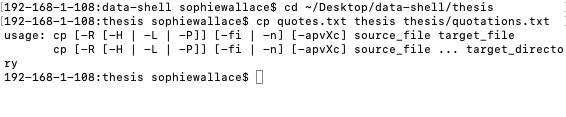
\includegraphics[width=\textwidth]{image1.png}

\subsection{Final Thoughts}
\textbf{6:20PM} Happy I was able to successfully insert the image into the document thanks to a friend. It would be really helpful to work in groups in class to understand errors and reiterate issues. The above image was the result from a previous exercise in Unix shell under "copying files and directories" in journal entry \textit{04/09/2019}. 

\section{05/09/2019}
\subsection{Elaboration Tests}
About to begin testing the tools described in elaboration II to examine whether they meet the specified criteria. Tools include: \textbf{Open Semantic Search} (\textbf{OPSS}), \textbf{Tropy} and \textbf{Excel + Cloudstor Sync Client (CSC).}
\subsection{Intention}
Answer the following questions regarding these tools:
\begin{itemize}
\item Is this tool compatible with both mobile and desktop?
\item Is this tool compatible with all data types?
\item Does this tool organise files with rich metadata?
\item Does this tool allow for editing of data?
\item Can this tool operate offline?
\item Does this tool have a reliable storage system?
\end{itemize}

\subsubsection{Open Semantic Search}
1:45PM Downloading OPSS
2:03PM Open and Upload OPSS
2:38PM Attempting to open OPSS with instructions from Brian and website link
2:45PM Open OPSS and begin tests

\subsubsection{Tropy}
2:17PM Moving onto Tropy tests

\subsection{Action}
\subsubsection{Open Semantic Search}
OSS Download
\begin{itemize}
\item Entered website
\item Clicked "Download Open Semantic Search"
\item Clicked "Open Semantiic Desktop Search"
\item Clicked hyperlink "Start Virtual Box"
\item Clicked "Download VirtualBox 6.0"
\item Clicked hyperlink "OS X Hosts" platform package 
\item \textbf{SUCCESS} package is downloading onto Mac 
\end{itemize}
Open and Upload OSS 
\begin{itemize}
\item Dragging VirtualBox item into Applications
\item Double click on VirtualBox from Applications 
\item Pop up box appears "This package will run a program to deteermine if the software can be installed"
\item Click continue
\item Oracle VM VirtualBox for macOS installer appears
\item Click continue
\item "This will take 258.5 MB of space on your computer" 
\item Click continue and proceeds to installation
\item \textbf{ERROR}: System Extention Blocked "A program tried to load new system extensions(s) signed by "Oracle . America,  Inc. if you want to enable these extensions, open Security and Privacy System Preferences" 
\item \textbf{ERROR}: The installation failed. "The Installer encountered an error that caused the installation to fail. Contact manufacturer for assistance"
\end{itemize}

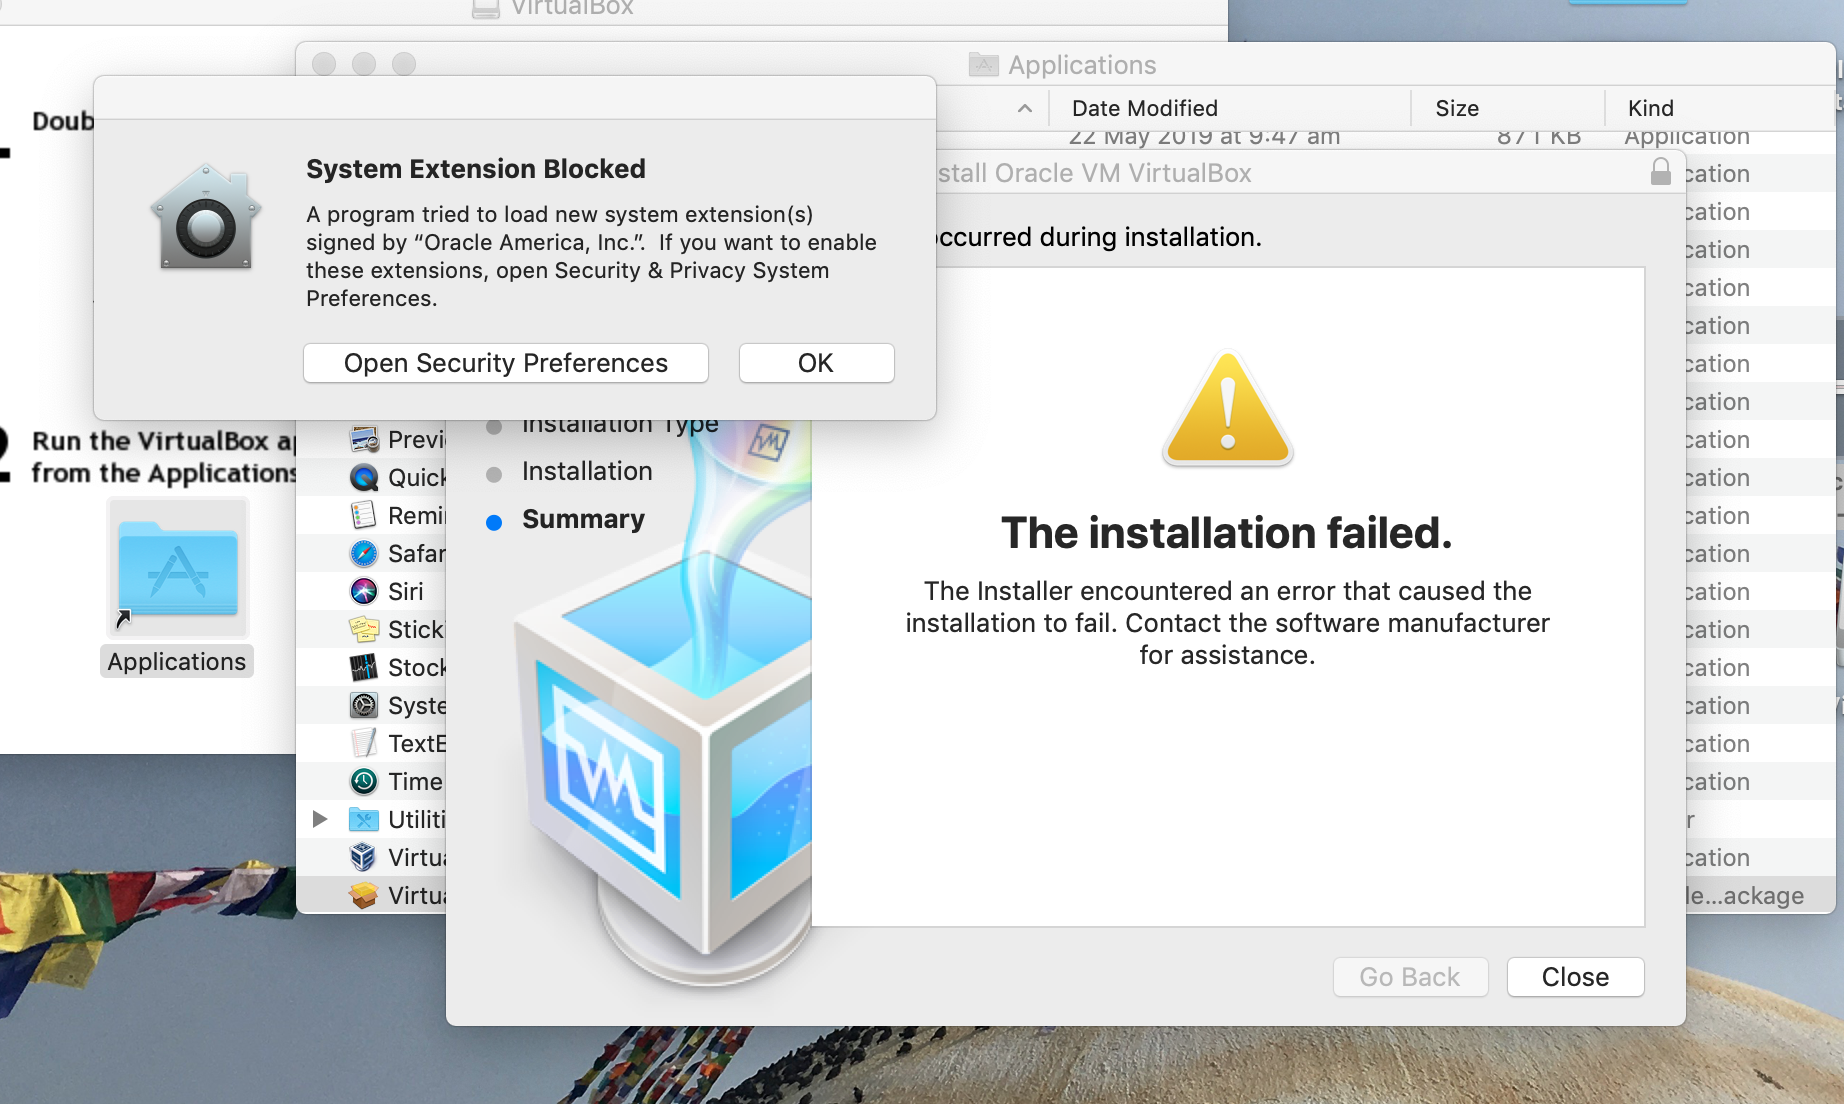
\includegraphics[width=\textwidth]{OSSfail.png}

Open and Upload OPSS
\begin{itemize}
\item Clicking through previous steps till I reach error
\item Quit out of the VirtualBox installer after fail
\item Open system preferences on mac
\item Choose "security and Privacy" 
\item Go to "General tab"
\item Click the lock button and enter administrator password
\item Click "allow" at the bottom of the security general section
\item Relaunch VirtualBox Installer (\textbf{SUCCESS})
\item Download the virtual machine image Open Semantic Desktop Search
\item Click on hyperlink "open-semantic-desktop-search19.07.19.ova (3 GB)"under multilingual section on Download page
\item Download is estimated 2 hours
\end{itemize}

Importing Files
\begin{itemize}
\item 
\end{itemize}



\subsection{Tropy}
\begin{itemize}
\item Click "Download Tropy for macOS"
\item 
\end{itemize}


\subsection{Final Thoughts}
\subsubsection{Open Semantic Search}
\textbf{2:10PM} I'm unsure about this download and don't want to get a virus or change my settings without being certain. I will share this journal with Brian to ask what he thinks. Excited I included the screenshot without needing to refer to prior notes though. \\
\textbf{3:02PM} Realised I had only downloaded VirtualBox, just one component of this software package. With download time estimated at 2 hours I will move back to Tropy.






















\end{document}
